\section{Study 5: Closed-Loop Vision Pipeline}
\label{sec:study5}

\subsection{Motivation}
\label{sec:study5:motivation}

In all previous studies, target coordinates $(P_x, P_y)$ are pre-specified numerically.
For real deployment, the robot must \emph{detect} the bin visually.
This study closes the perception loop by building two parallel vision pipelines ---
one classical (OpenCV) and one learning-based (YOLOv8n) --- and integrating each
with the trained throwing policy for end-to-end execution.

\subsection{OpenCV Geometric Pipeline}
\label{sec:study5:opencv}

\paragraph{Setup.}
A depth camera (emulated via PyBullet's \texttt{getCameraImage} with an RGB-D renderer)
is mounted on the arm base.
The bin is a hollow ring geometry modelled as a red object in the scene.

\paragraph{Detection.}
The pipeline proceeds in three steps:
\begin{enumerate}
  \item \textbf{HSV segmentation.} The RGB image is converted to HSV colour space and
        thresholded to isolate the red bin.
        Morphological operations (erosion + dilation) remove noise.
  \item \textbf{Contour centroid.} The largest contour is selected and its centroid
        pixel $(u, v)$ is computed via first-order moments.
  \item \textbf{Depth back-projection.} The depth value $d$ at $(u, v)$ is read from
        the depth buffer; the 3D point is recovered as
        $(x, y) = (d \cdot (u - c_x) / f_x,\; d \cdot (v - c_y) / f_y)$
        where $(c_x, c_y, f_x, f_y)$ are the camera intrinsics.
\end{enumerate}

\paragraph{Near-face bias correction.}
The camera sees the near face of the bin, not its centre.
The centroid of the visible rim arc lies at a distance $\approx 2R/\pi$ from the
bin centre, where $R$ is the bin radius.
The detected $(x, y)$ is shifted by $2R/\pi$ toward the centre of the detected
contour to compensate this systematic bias.

\paragraph{Failure handling.}
If HSV segmentation finds no contour above the minimum area threshold, the pipeline
falls back to a sampled target from the known target distribution and logs the detection
failure for offline analysis.

\subsection{YOLOv8n Learning-Based Pipeline}
\label{sec:study5:yolo}

\paragraph{Synthetic dataset.}
A dataset of 1{,}000 annotated images (800 training, 200 validation) is rendered in
PyBullet by randomising the camera pose, lighting, and bin position across the target
domain.
The bin is rendered as a red sphere at target height to standardise the detection
object class.
Bounding box annotations are generated programmatically from the projected bin
coordinates.

\paragraph{Training.}
YOLOv8n~\cite{yolov8} (nano variant, $\approx 3$\,M parameters) is trained on the synthetic dataset
for 50 epochs using the default Ultralytics training pipeline.
The model achieves mAP@0.5 $>$ 0.95 on the validation set.

\paragraph{Deployment.}
At inference time, the detected bounding box centroid $(u, v)$ plus the depth value $d$
at that pixel is back-projected to a 3D estimate $(x, y)$ via the same depth
back-projection as the OpenCV pipeline.
The YOLOv8n detection is more robust to partial occlusion and lighting variation than
HSV thresholding, at the cost of requiring a training dataset.

\subsection{End-to-End Integration}
\label{sec:study5:integration}

The full closed-loop pipeline executes as follows:
\begin{enumerate}
  \item The robot scans the workspace and captures an RGB-D frame.
  \item The vision pipeline (OpenCV or YOLO) detects the bin and estimates $(P_x, P_y)$.
  \item The trained policy $\pi_\theta(P_x, P_y)$ outputs release speed $v$.
  \item The throw executes: IK $\to$ spline $\to$ release $\to$ free flight.
  \item The ball enters the hollow bin (12-wall ring geometry in PyBullet).
\end{enumerate}

The bin in our simulator is modelled as a hollow ring composed of 12 rectangular walls
arranged in a cylinder, so the ball physically enters the bin rather than landing on a
flat surface.
This ensures that the vision-to-throw loop is evaluated under physically meaningful
entry conditions.

\subsection{Robustness to Camera Placement}
\label{sec:study5:robustness}

The depth back-projection assumes the camera intrinsics and extrinsics are known.
We test two camera positions: mounted on the arm base (default) and offset by 0.2\,m
laterally.
The near-face bias correction is recomputed for each camera position.
Both positions produce similar detection accuracy ($<$3\,cm offset in estimated
$(P_x, P_y)$ relative to ground truth), confirming that the pipeline does not
critically depend on a specific camera mount location.

\begin{figure}[t]
  \centering
  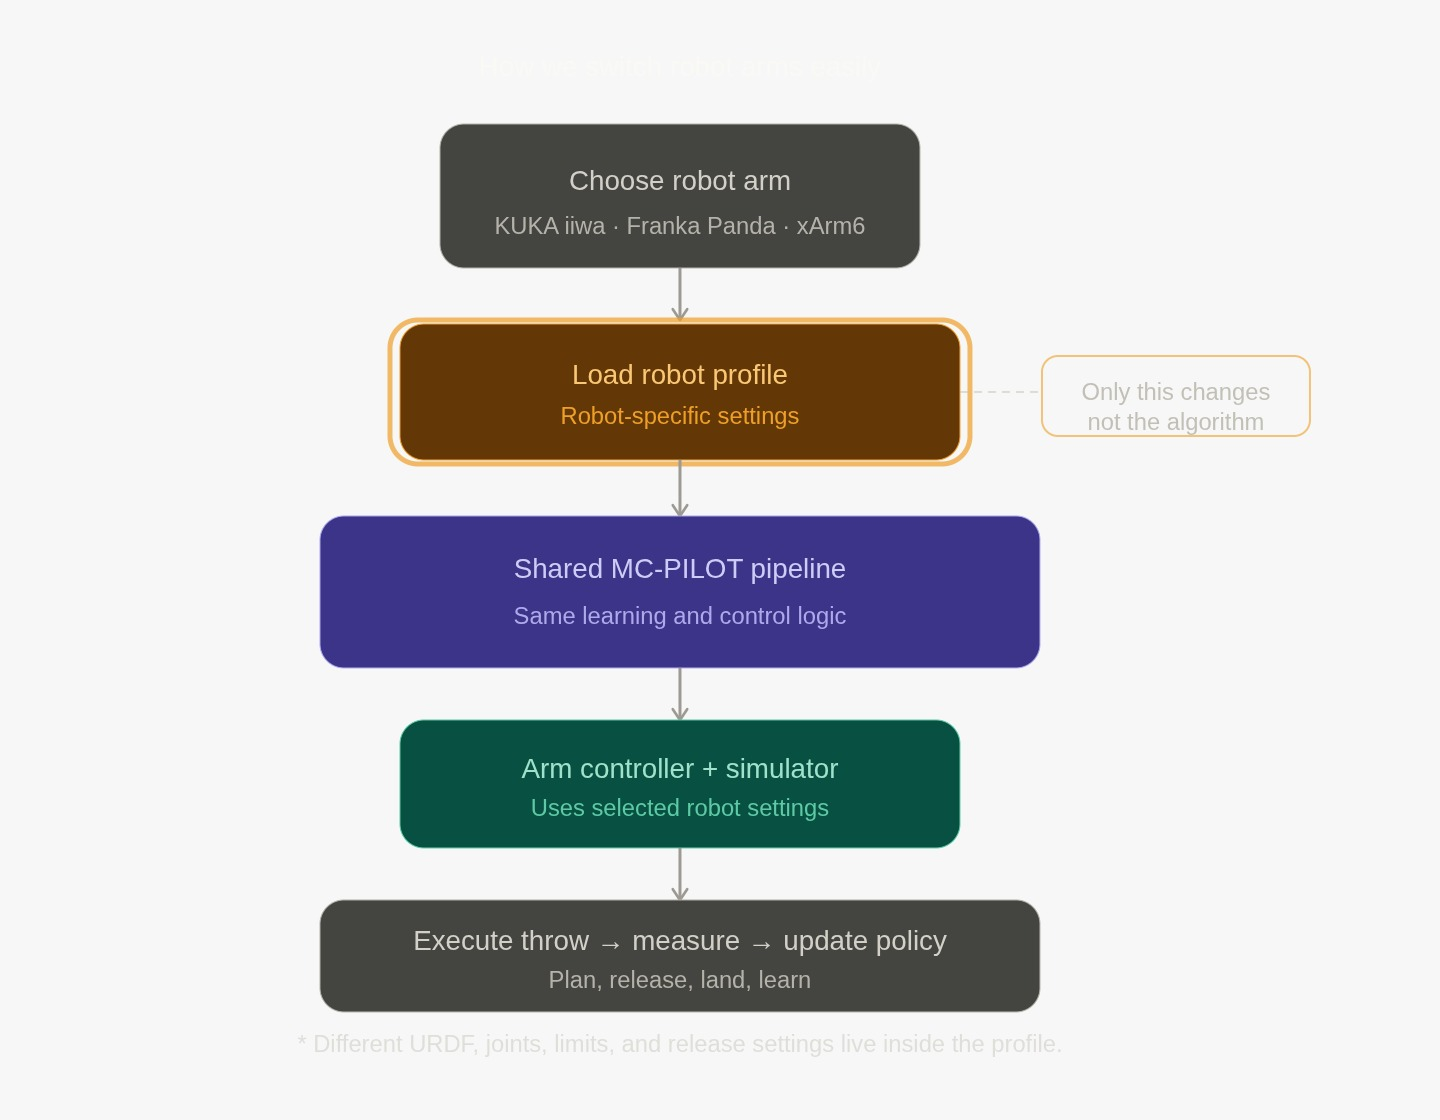
\includegraphics[width=\columnwidth]{../ppt/robot_arm_flowchart.jpeg}
  \caption{End-to-end system flowchart: perception (OpenCV or YOLO), policy inference,
           arm trajectory, and ball flight.}
  \label{fig:system_flowchart}
\end{figure}
